\documentclass[11pt]{amsart}
\usepackage{amsmath,amssymb,amsthm}
\usepackage[margin=1.15in]{geometry}
\usepackage{graphicx}
\usepackage[colorlinks=true,linkcolor=blue,citecolor=blue,urlcolor=blue]{hyperref}

\newtheorem{theorem}{Theorem}[section]
\newtheorem{lemma}[theorem]{Lemma}
\newtheorem{proposition}[theorem]{Proposition}
\newtheorem{corollary}[theorem]{Corollary}
\theoremstyle{remark}
\newtheorem{remark}[theorem]{Remark}

\newcommand{\Z}{\mathbb{Z}}
\newcommand{\Q}{\mathbb{Q}}
\newcommand{\C}{\mathbb{C}}
\newcommand{\F}{\mathbb{F}}
\newcommand{\N}{\mathrm{N}}
\newcommand{\fa}{\mathfrak{a}}
\newcommand{\fb}{\mathfrak{b}}
\newcommand{\fg}{\mathfrak{g}}
\newcommand{\fm}{\mathfrak{m}}
\newcommand{\fq}{\mathfrak{q}}
\newcommand{\fp}{\mathfrak{p}}
\newcommand{\Om}{\Omega}
\newcommand{\dd}{\mathrm{d}}
\newcommand{\cc}{\mathrm{c}}
\newcommand{\e}{\varepsilon}
\DeclareMathOperator{\li}{li}

\title[Level of distribution for orders of $y^2=x^3-x$ modulo $p$]{Recovering the level of distribution $x^{1/2}$ for the orders of $y^2=x^3-x$ modulo $p$}
\author{Ruqing Chen}
\address{GUT Geoservice Inc., Montreal, Canada}
\email{ruqing@hotmail.com}
\date{\today}

\begin{document}

\begin{abstract}
Iwaniec and Jim\'enez Urroz proved that for $\gg x/(\log x)^2$ primes $p\le x$, $p\equiv 1 \pmod 4$, the order of the reduction modulo $p$ of the curve $y^2=x^3-x$ is eight times an integer with at most two prime factors. Xie recently pointed out that the proof of their level-of-distribution estimate is incorrect: the inclusion--exclusion that converts a rational divisibility condition $d\mid \N(\pi-1)$ into congruences in $\Z[i]$ produces moduli of norm up to $d^2$, so that the Bombieri--Vinogradov theorem for $\Q(i)$ only gives level $x^{1/4-\e}$. We show that the estimate is nevertheless true at level $x^{1/2}(\log x)^{-B}$: the ideals of large norm are those with a large rational part, and their contribution is bounded trivially by counting lattice points. The same argument applies to the switched sequence used in the Chen-type part of the proof. Consequently the theorem of Iwaniec and Jim\'enez Urroz holds as stated, and Lemma~3.3 of Xie's paper holds with level $x^{1/2-\e}$; this improves her bounds for the orders over prime power fields, e.g.\ $|E(\F_{p^2})|/(4|E(\F_p)|)$ has at most three prime factors for $\gg x/(\log x)^2$ primes.
\end{abstract}

\maketitle

\section{Introduction}

Let $E$ be the elliptic curve $y^2=x^3-x$ over $\Q$, which has complex multiplication by $\Z[i]$. For a prime $p\equiv 1\pmod 4$ write $p=\pi\bar\pi$ with $\pi\in\Z[i]$ \emph{primary}, i.e.\ $\pi\equiv 1\pmod{2+2i}$; then $|E(\F_p)|=\N(\pi-1)$, and $8\mid \N(\pi-1)$. Koblitz \cite{Kob} conjectured that $|E(\F_p)|/8$ is prime for $\gg x/(\log x)^2$ primes $p\le x$, $p\equiv 1\pmod 4$. Sieve methods cannot reach primes, and the strongest result one can hope for is a Chen-type theorem. Iwaniec and Jim\'enez Urroz \cite[Theorem~1.2]{IJU} state:
\begin{equation}\label{eq:IJU}
\#\Bigl\{p\le x:\ p\equiv 1\ (\mathrm{mod}\ 4),\ \tfrac18|E(\F_p)| = P_2\Bigr\}\gg \frac{x}{(\log x)^2},
\end{equation}
where $P_r$ denotes a square-free integer with at most $r$ prime factors. The proof follows Chen's method in $\Z[i]$: a weighted linear sieve applied to the sequence $\mathcal A(x)=\{\N(\pi-1)/8\}$ (\cite[\S\S 3--4]{IJU}) and a switching argument applied to the sequence $\mathcal B(x)=\{\N(1+\omega)\}$, where $\omega$ runs over products of three Gaussian primes in prescribed ranges (\cite[\S 5]{IJU}). Both sieves need the level of distribution $x^{1/2}(\log x)^{-B}$, that is, estimates of the form
\begin{equation}\label{eq:level}
\sum_{d\le x^{1/2}(\log x)^{-B}}\mu^2(d)\,3^{\omega(d)}\,|r_d(x)|\ll \frac{x}{(\log x)^A},
\end{equation}
where $r_d(x)$ is the error in the number of elements of the sequence divisible by $d$; these are (3.9) and (5.9) of \cite{IJU}.

In a recent paper on almost prime orders over prime power fields, Xie \cite[Remark~4.1]{Xie} observed that the derivation of \cite[(3.9)]{IJU} from the Bombieri--Vinogradov theorem for $\Q(i)$ is incorrect. The point is the following. A square-free $d$ divides $\N(\alpha)$ if and only if, for each inert prime $q\mid d$, $q\mid\alpha$, and for each split prime $p=\pi_p\bar\pi_p$ dividing $d$, $\pi_p\mid\alpha$ or $\bar\pi_p\mid\alpha$. Inclusion--exclusion turns $d\mid \N(\alpha)$ into a signed sum of conditions $\fa\mid\alpha$ over the ideals $\fa=\prod_{q\mid d}(q)\prod_{p\mid d}\fa_p$ with $\fa_p\in\{(\pi_p),(\bar\pi_p),(p)\}$, and $\N(\fa)$ ranges between $d$ and $d^2$. The Bombieri--Vinogradov theorem for $\Q(i)$ controls moduli of norm up to $x^{1/2}(\log x)^{-B}$, which only gives \eqref{eq:level} with $d\le x^{1/4}(\log x)^{-B}$. (In \cite[p.~823]{IJU} the terms with $\fa_p=(p)$ are lost in the passage from ideals to integers; Xie's Lemma~3.3 keeps them and obtains level $x^{1/4-\e}$.) Xie concludes that \eqref{eq:IJU} is not established by \cite{IJU}, and that the best unconditional result is $P_5$ \cite{Coj, Xie}.

The purpose of this note is to show that \eqref{eq:level} is true at level $x^{1/2}(\log x)^{-B}$ for both sequences, so that the argument of \cite{IJU} is complete. The idea is simple. Write a square-free ideal $\fa$ as $\fa=(c)\fg$ with $c\in\Z_{>0}$ as large as possible (the \emph{rational part} of $\fa$) and $\fg$ primitive. Then $d=c\,\N(\fg)$ and $\N(\fa)=c\,d$. The ideals of large norm are exactly those with a large rational part, and these are rare: the expected number of elements of the sequence in a residue class modulo $\fa$ is of size $x/\N(\fa)=x/(cd)$, which is summable over $c$. For $c\le(\log x)^{B_0}$ we have $\N(\fa)\le (\log x)^{B_0} d$, which is within reach of the Bombieri--Vinogradov theorem; for $c>(\log x)^{B_0}$ the contribution is bounded trivially by counting lattice points in a disc. This is in fact the mechanism already used in \cite[p.~823]{IJU} to discard the inert primes, which contribute $q^2$ to the norm; the split primes with $\fa_p=(p)$ have to be treated in the same way.

We state the result in a form that applies to any sequence for which a Bombieri--Vinogradov theorem over ideals is available (Theorem~\ref{thm:main}), and then apply it to the two sequences of \cite{IJU} (Section~\ref{sec:appl}). The same statement holds over any imaginary quadratic field of class number one (Remark~\ref{rem:classnumber}), which is the setting of the extension of \cite{IJU} to all CM curves over $\Q$ in \cite{JU}. As a by-product, the level $x^{1/2-\e}$ in Lemma~3.3 of \cite{Xie} improves the almost-prime bounds of \cite[Theorem~1.3]{Xie} for $|E(\F_{p^\ell})|/|E(\F_p)|$ (Corollary~\ref{cor:Xie}). Section~\ref{sec:rest} records a few remarks on the remaining parts of \cite{IJU}, in particular on the hypothesis of their Lemma~5.2. The code and data behind the numerical statements are described at the end of the paper (GitHub repository; the manuscript is archived at Zenodo, \href{https://doi.org/10.5281/zenodo.23428952}{doi:10.5281/zenodo.23428952}).

\subsection*{Acknowledgement} I thank Likun Xie for her comments on a first version of the argument.

\section{The main lemma}\label{sec:main}

Throughout, $\N(\alpha)=|\alpha|^2$ is the norm on $\Z[i]$, ideals are denoted by fraktur letters, $\Phi(\fm)=|(\Z[i]/\fm)^\times|$, and $L=\log x$. Every ideal of $\Z[i]$ is principal.

\subsection{Lattice points in a residue class}

\begin{lemma}\label{lem:lattice}
Let $\fm=(\gamma)\neq 0$ be an ideal of $\Z[i]$, $\alpha\in\Z[i]$ and $r>0$. Then
\[
\#\{w\in\alpha+\fm:\ |w|\le r\}\le\Bigl(\frac{2r}{\N(\fm)^{1/2}}+1\Bigr)^2\ll \frac{r^2}{\N(\fm)}+1.
\]
\end{lemma}

\begin{proof}
The set $\alpha+\fm=\alpha+\gamma\Z[i]$ is a translate of the lattice $\gamma\Z[i]\subset\C$, whose nonzero vectors have length at least $\lambda=|\gamma|=\N(\fm)^{1/2}$. The open discs of radius $\lambda/2$ centred at the points of $\alpha+\fm$ are pairwise disjoint, and those centred at points of modulus $\le r$ are contained in the disc of radius $r+\lambda/2$. Comparing areas gives the bound $(r+\lambda/2)^2/(\lambda/2)^2$.
\end{proof}

\subsection{The rational part of a square-free ideal}

For an ideal $\fa\ne 0$ let $\dd(\fa)$ be the least positive rational integer in $\fa$, and let $\cc(\fa)$ be the largest positive rational integer $c$ with $(c)\supseteq\fa$. Then $\fa=(\cc(\fa))\,\fg$ where $\fg$ is \emph{primitive}, i.e.\ not divisible by any rational integer $>1$.

\begin{lemma}\label{lem:rational}
Let $\fa$ be a square-free ideal, $c=\cc(\fa)$ and $\fa=(c)\fg$. Then $c$ is odd and square-free, $\dd(\fa)=c\,\N(\fg)$, and
\[
\N(\fa)=\cc(\fa)\,\dd(\fa).
\]
Moreover, for a square-free integer $d\ge 1$ the square-free ideals $\fa$ with $\dd(\fa)=d$ are exactly the ideals
\[
\fa=(1+i)^{e}\prod_{q\mid d}(q)\prod_{p\mid d}\fa_p,\qquad e=1 \text{ if } 2\mid d,\ e=0 \text{ otherwise},\qquad \fa_p\in\{(\pi_p),(\bar\pi_p),(p)\},
\]
where $q$ runs over the primes $\equiv 3\pmod 4$ and $p=\pi_p\bar\pi_p$ over the primes $\equiv 1\pmod 4$ dividing $d$. In particular their number is $3^{\omega_1(d)}\le 3^{\omega(d)}$, where $\omega_1(d)$ is the number of prime factors $p\equiv 1\pmod 4$ of $d$, and $\cc(\fa)=\prod_{q\mid d}q\prod_{\fa_p=(p)}p$ divides $d$.
\end{lemma}

\begin{proof}
Since $\fa$ is square-free and $(2)=(1+i)^2$, no even integer $c$ satisfies $(c)\supseteq\fa$, and $c$ is square-free. A rational integer $n$ lies in $\fg$ if and only if every prime ideal factor $\fp$ of $\fg$ divides $n$; for $\fp=(\pi_p)$ or $(\bar\pi_p)$ this means $p\mid n$ (as $n=\bar n$), for $\fp=(q)$ it means $q\mid n$, and for $\fp=(1+i)$ it means $2\mid n$. Since $\fg$ is primitive and square-free, no two of its prime ideal factors lie above the same rational prime, so $n\in\fg$ if and only if $\N(\fg)\mid n$, i.e.\ $\dd(\fg)=\N(\fg)$. Now $n\in(c)\fg$ if and only if $c\mid n$ and $n/c\in\fg$, so $\dd(\fa)=c\,\N(\fg)$, and $\N(\fa)=c^2\N(\fg)=c\,\dd(\fa)$. The description of the ideals with $\dd(\fa)=d$ follows from $\dd(\fa)=\prod_{\fp\mid\fa}\dd(\fp)$ for square-free $\fa$ (the primes above different rational primes being coprime), with $\dd((\pi_p))=\dd((\bar\pi_p))=\dd((p))=p$, $\dd((q))=q$, $\dd((1+i))=2$, and $(2)$ being excluded as not square-free.
\end{proof}

\subsection{From norm to least integer}

\begin{theorem}\label{thm:main}
Let $x\ge 3$ and let $R(\fm)\ge 0$ be a function on the nonzero ideals of $\Z[i]$ such that
\begin{enumerate}
\item[\textup{(i)}] for every $A>0$ there is $B=B(A)>0$ with
\[
\sum_{\N(\fm)\le x^{1/2}L^{-B}}R(\fm)\ll_A \frac{x}{L^{A}};
\]
\item[\textup{(ii)}] $R(\fm)\ll x L/\N(\fm)+1$ for every $\fm$ with $\N(\fm)\le x$.
\end{enumerate}
Let $\fb$ be a fixed nonzero ideal and $k\ge 0$. Then for every $A>0$ there is $B'=B'(A,k,\fb)$ such that
\[
\sum_{\substack{\fa\ \mathrm{square\text{-}free}\\ \dd(\fa)\le x^{1/2}L^{-B'}}}\tau(\dd(\fa))^{k}\,R(\fb\fa)\ll_{A,k,\fb} \frac{x}{L^{A}}.
\]
\end{theorem}

\begin{proof}
Put $D=x^{1/2}L^{-B'}$ and $C_0=L^{B_0}$, with $B_0,B'$ to be chosen. Note that every ideal in the sum satisfies $\N(\fb\fa)=\N(\fb)\cc(\fa)\dd(\fa)\le\N(\fb)D^2\le x$ for $x$ large, since $\cc(\fa)\le\dd(\fa)$; so hypothesis (ii) is available throughout. Split the sum according to whether $\cc(\fa)\le C_0$ or $\cc(\fa)>C_0$.

\emph{Ideals with small rational part.} If $\cc(\fa)\le C_0$ and $\dd(\fa)\le D$, then by Lemma~\ref{lem:rational}
\[
\N(\fb\fa)=\N(\fb)\,\cc(\fa)\,\dd(\fa)\le \N(\fb)\,C_0 D\le x^{1/2}L^{-B}
\]
provided $B'\ge B+B_0+1$ and $x$ is large in terms of $\fb$, where $B=B(A_1)$ with $A_1$ to be chosen. Since $\fa\mapsto\fb\fa$ is injective and $R\ge 0$, hypothesis (i) gives $\sum R(\fb\fa)\ll xL^{-A_1}$ over this family. To insert the weight $\tau(\dd(\fa))^k$ we use Cauchy's inequality together with the trivial bound (ii):
\[
\sum \tau(\dd(\fa))^{k}R(\fb\fa)\le\Bigl(\sum\tau(\dd(\fa))^{2k}R(\fb\fa)\Bigr)^{1/2}\Bigl(\sum R(\fb\fa)\Bigr)^{1/2},
\]
and, grouping the ideals according to $d=\dd(\fa)$ (at most $3^{\omega(d)}$ ideals for each $d$) and using $\N(\fb\fa)\ge\dd(\fa)$,
\[
\sum\tau(\dd(\fa))^{2k}R(\fb\fa)\ll\sum_{d\le D}\tau(d)^{2k}3^{\omega(d)}\Bigl(\frac{xL}{d}+1\Bigr)\ll x L^{c_k}
\]
for some $c_k$ depending only on $k$. Hence the ideals with small rational part contribute $\ll x L^{(c_k-A_1)/2}$, which is $\ll xL^{-A}$ for $A_1=2A+c_k$.

\emph{Ideals with large rational part.} For $\cc(\fa)>C_0$ we use (ii) and $\N(\fb\fa)\ge\N(\fa)=\cc(\fa)\dd(\fa)>C_0\,\dd(\fa)$, so that $R(\fb\fa)\ll xL/(C_0\dd(\fa))+1$. Grouping again according to $d=\dd(\fa)$ (at most $3^{\omega(d)}$ ideals for each $d$), the contribution is
\[
\ll\sum_{d\le D}\tau(d)^k\,3^{\omega(d)}\Bigl(\frac{xL}{C_0d}+1\Bigr)
\ll \frac{x L^{c'_k}}{C_0}+D L^{c'_k},
\]
which is $\ll xL^{-A}$ once $B_0=A+c'_k$. This proves the theorem with $B'=B(2A+c_k)+A+c'_k+1$.
\end{proof}

\begin{remark}\label{rem:weak}
The hypothesis (ii) is a trivial bound, satisfied by every $R$ that arises as the discrepancy of a set of Gaussian integers of norm $\le x$ in residue classes, by Lemma~\ref{lem:lattice}. The proof uses (ii) only inside sums carrying divisor-function weights, so (ii) may be weakened to $R(\fm)\ll\tau(\N(\fm))^{c_0}\,(xL/\N(\fm)+1)$ for a fixed $c_0$, at the cost of changing $c_k, c'_k$: for $\fm=\fb\fa$ with $\dd(\fa)=d$ one has $\N(\fm)\mid \N(\fb)d^2$, hence $\tau(\N(\fm))\le\tau(\N(\fb))\tau(d)^2$. This covers sets defined by a condition $\fa\mid\Phi(\pi)$ with $\Phi$ a polynomial, where the number of admissible residue classes modulo $\fa$ is $\ll\deg(\Phi)^{\omega(\fa)}$. Hypothesis (i) is a Bombieri--Vinogradov theorem over ideals of norm up to $x^{1/2}L^{-B}$. The conclusion is a Bombieri--Vinogradov theorem over ideals of \emph{least integer} up to $x^{1/2}L^{-B'}$, which is what a rational sieve applied to $\N(\alpha)$ needs. Nothing is lost: in the main term of the sieve the ideals with large rational part contribute $\ll xL^{O(1)}/C_0$ as well, so they are negligible on both sides.
\end{remark}

\begin{remark}\label{rem:classnumber}
Lemmas~\ref{lem:lattice} and \ref{lem:rational} and Theorem~\ref{thm:main} hold for the ring of integers $\mathcal O_K$ of any imaginary quadratic field $K$ of class number one, with $\Z[i]$ replaced by $\mathcal O_K\subset\C$ and with one change of wording: every ideal $(\gamma)$ is a lattice with minimal distance $|\gamma|=\N(\gamma)^{1/2}$, and the decomposition $\fa=(c)\fg$ with $\N(\fa)=c\,\dd(\fa)$ holds for square-free $\fa$, where now $c$ is square-free and coprime to the discriminant of $K$ (a ramified prime $(p)=\fp^2$ occurs at most once in $\fa$ and contributes its norm $p$ to $\dd(\fg)=\N(\fg)$; in $\Z[i]$ the only ramified prime is $2$, whence ``$c$ is odd'' in Lemma~\ref{lem:rational}). This is the setting of the extension of \cite{IJU} to all CM curves over $\Q$ in \cite{JU}, which follows the argument of \cite{IJU} and is therefore affected by the same gap; Theorem~\ref{thm:main} supplies the missing estimate there as well, but we have not checked the remaining details of \cite{JU}.
\end{remark}

\section{Application to the two sequences of Iwaniec and Jim\'enez Urroz}\label{sec:appl}

We keep the notation of \cite{IJU}: $z=x^{1/8}$, $y=x^{1/3}$, and $\pi_1,\pi_2,\pi_3$ denote primary Gaussian primes above split rational primes, $\N(\pi_j)=p_j\equiv 1\pmod 4$. A primary prime $\pi$ is either of this kind or $\pi=-q$ with $q\equiv 3\pmod 4$ inert; there are $O(x^{1/2})$ of the latter with $\N(\pi)\le x$, and we include them in the sequence $\mathcal A(x)$ below (see the comment after Corollary~\ref{cor:A}).

\subsection{Inclusion--exclusion}
For $\alpha\in\Z[i]$ and a prime $\ell$ we have: $2\mid\N(\alpha)$ iff $(1+i)\mid\alpha$; for $q\equiv 3\pmod 4$, $q\mid\N(\alpha)$ iff $q\mid\alpha$; for $p=\pi_p\bar\pi_p\equiv 1\pmod 4$, $p\mid\N(\alpha)$ iff $\pi_p\mid\alpha$ or $\bar\pi_p\mid\alpha$, so that
\[
\mathbf 1_{p\mid\N(\alpha)}=\mathbf 1_{\pi_p\mid\alpha}+\mathbf 1_{\bar\pi_p\mid\alpha}-\mathbf 1_{p\mid\alpha}.
\]
Multiplying over the prime factors of a square-free $d$ and using Lemma~\ref{lem:rational} we obtain
\begin{equation}\label{eq:ie}
\mathbf 1_{d\mid\N(\alpha)}=\sum_{\substack{\fa\ \mathrm{square\text{-}free}\\ \dd(\fa)=d}}(-1)^{r(\fa)}\,\mathbf 1_{\fa\mid\alpha},\qquad r(\fa)=\#\{p\mid d:\ \fa_p=(p)\}.
\end{equation}
This is \cite[Lemma~3.1 and (3.12)]{Xie}. Define the multiplicative function $\hat g$ on square-free ideals by $\hat g(\fa)=4/\Phi((2+2i)\fa)$, so that $\hat g((1+i))=1/2$, $\hat g((\pi_p))=\hat g((\bar\pi_p))=1/(p-1)$, $\hat g((q))=1/(q^2-1)$, and
\begin{equation}\label{eq:g}
g(d)=\sum_{\dd(\fa)=d}(-1)^{r(\fa)}\hat g(\fa)=\prod_{\ell\mid d}g(\ell),\qquad g(2)=\tfrac12,\quad g(q)=\frac{1}{q^2-1},\quad g(p)=\frac{2}{p-1}-\frac{1}{(p-1)^2},
\end{equation}
which is the density function of \cite[(3.7)]{IJU}.

\subsection{The sequence $\mathcal A(x)$}
Let $\Pi^*(x)$ be the number of prime elements $\pi\in\Z[i]$ (all associates counted) with $\N(\pi)\le x$, and for an ideal $\fq$ and $\alpha\in\Z[i]$ let $\Pi(x;\fq,\alpha)$ be the number of those with $\pi\equiv\alpha\pmod\fq$. The Bombieri--Vinogradov theorem for $\Q(i)$ (Huxley \cite[Theorem~1]{Hux71}, stated there for reduced narrow ideal classes of a number field; the form below for residue classes in $\Z[i]$ is \cite[Proposition~2.2]{Xie} and \cite[Proposition~3.2]{IJU}; see also Johnson \cite[Corollary]{Joh} and Hinz \cite{Hinz}) states that for every $A$ there is $B$ with
\begin{equation}\label{eq:BV}
\sum_{\N(\fq)\le x^{1/2}L^{-B}}\ \max_{(\alpha,\fq)=1}\Bigl|\Pi(x;\fq,\alpha)-\frac{\Pi^*(x)}{\Phi(\fq)}\Bigr|\ll\frac{x}{L^{A}}.
\end{equation}
(For $\N(\fq)\le 4$ the terms are trivially $O(x^{1/2})$; for $\N(\fq)>4$ the four units are distinct modulo $\fq$, so counting prime elements in a class is the same as counting prime ideals with a generator in that class, as in \cite[Proposition~2.2]{Xie}.)
Let $X=\Pi^*(x)/4$; this is the number of prime ideals of norm $\le x$, and $X=\Pi(x)+O(x^{1/2})$ in the notation of \cite{IJU}, where $\Pi(x)$ counts the primary primes above split $p\le x$. For square-free $d$ let
\[
A_d(x)=\#\{\pi\ \text{primary}:\ \N(\pi)\le x,\ d\mid \N(\pi-1)/8\}.
\]
Since $\pi$ is primary, $\alpha=(\pi-1)/(2+2i)\in\Z[i]$ and $\N(\alpha)=\N(\pi-1)/8$; moreover $\fa\mid\alpha$ if and only if $\pi\equiv 1\pmod{(2+2i)\fa}$, and the condition $\pi\equiv1\pmod{2+2i}$ is then automatic. Hence by \eqref{eq:ie}
\[
A_d(x)=\sum_{\dd(\fa)=d}(-1)^{r(\fa)}\,\Pi\bigl(x;(2+2i)\fa,1\bigr)=X g(d)+r_d(x),\qquad |r_d(x)|\le\sum_{\dd(\fa)=d}R_{\mathcal A}((2+2i)\fa),
\]
where $R_{\mathcal A}(\fq)=\max_{(\alpha,\fq)=1}|\Pi(x;\fq,\alpha)-\Pi^*(x)/\Phi(\fq)|$. Hypothesis (i) of Theorem~\ref{thm:main} for $R_{\mathcal A}$ is \eqref{eq:BV}; hypothesis (ii) follows from Lemma~\ref{lem:lattice}, which gives $\Pi(x;\fq,\alpha)\ll x/\N(\fq)+1$, and from $\Phi(\fq)\gg\N(\fq)/\log\log\N(\fq)$. Theorem~\ref{thm:main} with $\fb=(2+2i)$ and $k=2$ (note $3^{\omega(d)}\le\tau(d)^2$) gives:

\begin{corollary}\label{cor:A}
For every $A>0$ there is $B'>0$ such that
\[
\sum_{d\le x^{1/2}L^{-B'}}\mu^2(d)\,3^{\omega(d)}\,|r_d(x)|\ll\frac{x}{L^{A}}.
\]
\end{corollary}

This is \cite[(3.9)]{IJU}, with the weight $3^{\omega(d)}$ required by the Jurkat--Richert theorem in the form of \cite[Theorem~8.4]{HR}. (In \cite{IJU} the sequence $\mathcal A(x)$ is indexed by the primary primes above split $p$ only; our $A_d(x)$ also counts the $O(x^{1/2})$ primary primes $-q$, $q\equiv3\pmod 4$, $q\le x^{1/2}$, for which the identity above is exact. Removing them changes the sifted sum by at most $O(x^{1/2})$, which is negligible against $x/(\log x)^2$.) It is also Lemma~3.3 of \cite{Xie} with the condition $(d_1d_2)^2\le x^{1/2}L^{-B}$ replaced by $d_1d_2\le x^{1/2}L^{-B'}$ (the vector-sieve remainder of \cite[Proposition~2.8]{Xie} involves the same family of moduli).

\subsection{The switched sequence $\mathcal B(x)$}
Let
\[
\Om(x)=\bigl\{\omega=(1+i)^3\e\,\pi_1\pi_2\pi_3:\ \e\in\{\pm1,\pm i\},\ \N(\omega)\le x,\ z\le\N(\pi_3)<y\le\N(\pi_2)<\N(\pi_1)\bigr\}.
\]
Since the norms of $\pi_1,\pi_2,\pi_3$ are distinct, no conjugate pair occurs among them, and by unique factorisation the map $\omega\mapsto(\e,\pi_1,\pi_2,\pi_3)$ is injective; thus $\Om(x)$ is a set of $\ll x$ Gaussian integers of norm $\le x$, each counted once. All elements $1+\omega$ are coprime to $1+i$, so $\N(1+\omega)$ is odd. For an odd ideal $\fm$ and $(\alpha,\fm)=1$ put
\[
E(x;\alpha,\fm)=\#\{\omega\in\Om(x):\ \omega\equiv\alpha\ (\mathrm{mod}\ \fm)\}-\frac{1}{\Phi(\fm)}\#\{\omega\in\Om(x):\ (\omega,\fm)=1\},
\]
and $R_{\mathcal B}(\fm)=\max_{(\alpha,\fm)=1}|E(x;\alpha,\fm)|$ for odd $\fm$, $R_{\mathcal B}(\fm)=0$ for even $\fm$ (both counts vanish then). Proposition~5.1 of \cite{IJU} is the statement that $R_{\mathcal B}$ satisfies hypothesis (i) of Theorem~\ref{thm:main}; see Section~\ref{sec:rest} for its proof. Hypothesis (ii) is again Lemma~\ref{lem:lattice}, since $|E(x;\alpha,\fm)|\le\#\{w\in\alpha+\fm:\N(w)\le x\}+|\Om(x)|/\Phi(\fm)$.

For odd square-free $d$ let $B_d(x)=\#\{\omega\in\Om(x): d\mid\N(1+\omega)\}$. By \eqref{eq:ie} with $\alpha=1+\omega$,
\[
B_d(x)=\sum_{\dd(\fa)=d}(-1)^{r(\fa)}\#\{\omega\in\Om(x):\ \omega\equiv-1\ (\mathrm{mod}\ \fa)\}
=|\Om(x)|\,g(d)+r^{\mathcal B}_d(x),
\]
where now, since $\Phi(\fa)^{-1}=\hat g(\fa)$ for odd $\fa$,
\[
r^{\mathcal B}_d(x)=\sum_{\dd(\fa)=d}(-1)^{r(\fa)}\Bigl(E(x;-1,\fa)-\frac{1}{\Phi(\fa)}\#\{\omega\in\Om(x):\ (\omega,\fa)\ne1\}\Bigr).
\]
The first part is handled by Theorem~\ref{thm:main} with $\fb=(1)$. For the second part note that $(\omega,\fa)\neq 1$ forces some $\pi_j\mid\fa$, with $\N(\pi_j)\ge z$, and for a fixed prime $\pi$ the number of $\omega\in\Om(x)$ divisible by $\pi$ is at most $4\#\{\beta:\N(\beta)\le x/(8\N(\pi))\}\ll x/\N(\pi)$. Hence, writing $\fa=(\pi)\fa'$,
\[
\sum_{\dd(\fa)\le D}3^{\omega(\dd(\fa))}\frac{\#\{\omega:(\omega,\fa)\ne1\}}{\Phi(\fa)}
\ll x\sum_{\N(\pi)\ge z}\frac{1}{\N(\pi)\Phi((\pi))}\sum_{\N(\fa')\le D^2}\frac{3^{\omega(\dd(\fa'))}}{\Phi(\fa')}\ll\frac{xL^{c}}{z}.
\]

\begin{corollary}\label{cor:B}
For every $A>0$ there is $B'>0$ such that
\[
\sum_{\substack{d\le x^{1/2}L^{-B'}\\ d\ \mathrm{odd}}}\mu^2(d)\,3^{\omega(d)}\,|r^{\mathcal B}_d(x)|\ll\frac{x}{L^{A}}.
\]
\end{corollary}

This is \cite[(5.9)]{IJU}, whose derivation from Proposition~5.1 there is said to be ``the same as the one done to go from (3.8) to (3.9)'' and therefore had the same gap.

\subsection{Conclusion}
Corollaries~\ref{cor:A} and \ref{cor:B} are precisely the inputs \cite[(3.9) and (5.9)]{IJU} needed for the three sieve estimates \cite[(3.13), (4.3), (5.10)]{IJU}, namely
\begin{gather*}
W_1(x)\ge\Bigl(\tfrac12e^{\gamma}\log 3-\e\Bigr)\Pi(x)V(z),\qquad
W_2(x)\le\Bigl(\tfrac12e^{\gamma}\log 6+\e\Bigr)\Pi(x)V(z),\\
W_3(x)\le\Bigl(\tfrac12e^{\gamma}c+\e\Bigr)\Pi(x)V(z),\qquad
c=\int_{1/8}^{1/3}\int_{1/3}^{(1-u)/2}\frac{\dd u\,\dd v}{uv(1-u-v)}=0.36308372\ldots,
\end{gather*}
and therefore
\begin{align*}
W_1-\tfrac12W_2-\tfrac12W_3&\ge\tfrac12 e^{\gamma}\bigl(\log 3-\tfrac12\log 6-\tfrac12 c-3\e\bigr)\Pi(x)V(z)\\
&=\tfrac12 e^{\gamma}(0.02119\ldots-3\e)\,\Pi(x)V(z)>0 .
\end{align*}
Hence \eqref{eq:IJU} holds: \emph{Theorem~1.2 of \cite{IJU} is correct as stated.}

\subsection{Orders over prime power fields}
Theorem~\ref{thm:main} also raises the level of distribution in the prime-power results of \cite{Xie}. For an odd prime $\ell$, $|E(\F_{p^\ell})|/|E(\F_p)|=\N(\Phi_\ell(\pi))$ with $\Phi_\ell$ the $\ell$-th cyclotomic polynomial, and for $\ell=2$, $|E(\F_{p^2})|/(4|E(\F_p)|)=\N(\pi+1)/4$. In \cite[\S4]{Xie} these sequences are sifted with a weighted linear sieve whose remainder is controlled by \cite[(4.6)]{Xie}, an estimate of the form \eqref{eq:level} at level $x^{1/4-\e}$ deduced from the Bombieri--Vinogradov theorem over ideals \cite[(4.3)]{Xie} through $d\le\N(\fa)\le d^2$. Theorem~\ref{thm:main} (with Remark~\ref{rem:weak}, since $\fa\mid\Phi_\ell(\pi)$ is a union of at most $(\ell-1)^{\omega(\fa)}$ residue classes modulo $\fa$) gives \cite[(4.6)]{Xie} at level $x^{1/2}L^{-B'}$ instead. The weighted sieve of \cite[(4.7)--(4.9)]{Xie} then yields, for $\gg x/(\log x)^2$ primes $p\le x$, $p\equiv1\pmod 4$,
\[
\Omega(a)\le\Bigl\lfloor\frac1\lambda+\frac{\ell-1}{\delta}\Bigr\rfloor\qquad\text{whenever }0<\theta<\delta<\alpha\text{ and } G(\theta,\delta,\lambda)>0,
\]
where
\[
G(\theta,\delta,\lambda)=f\Bigl(\frac\alpha\theta\Bigr)-\lambda\int_\theta^\delta F\Bigl(\frac{\alpha-t}{\theta}\Bigr)\Bigl(1-\frac t\delta\Bigr)\frac{\dd t}{t},
\]
now with $\alpha=1/2-\e$, where $f$, $F$ are the lower and upper bound functions of the linear sieve, $F(s)=2e^\gamma/s$ for $0<s\le3$ and $f(s)=2e^\gamma\log(s-1)/s$ for $2\le s\le 4$.\footnote{In \cite[(4.11)]{Xie} the value $F(s)=2e^{\gamma}$ is used for $0<s<1$. The upper bound sieve at level $D<z$ is obtained by sifting only by the primes below $D$, which gives $F(s)=2e^{\gamma}/s$ also for $0<s<1$; the value $2e^\gamma$ is not an admissible upper bound there. With $F(s)=2e^\gamma/s$ the quantity $G(1/15,1/4.1,1/1.3)$ at level $1/4.01$ in \cite{Xie} equals $0.0676$ rather than $0.1341$; it is still positive, so the conclusions of \cite[\S4]{Xie} are unaffected.} We choose $\alpha/4\le\theta<\delta<\alpha$, so that $3\le\alpha/\theta\le4$ and $0<(\alpha-t)/\theta\le3$ on the whole range of integration; then only the closed forms are needed, and partial fractions give
\[
G(\theta,\delta,\lambda)=\frac{2e^\gamma\theta}{\alpha}\Bigl[\log\Bigl(\frac\alpha\theta-1\Bigr)-\lambda\Bigl(\log\frac\delta\theta-\Bigl(\frac\alpha\delta-1\Bigr)\log\frac{\alpha-\theta}{\alpha-\delta}\Bigr)\Bigr].
\]
At $\alpha=0.499$, $\theta=1/8$ this gives (interval arithmetic, but the reader may check it with a pocket calculator)
\[
G\bigl(\tfrac18,\tfrac9{20},\tfrac{10}{17}\bigr)= 0.4217\ldots>0,\qquad G\bigl(\tfrac18,\tfrac{20}{41},\tfrac56\bigr)= 0.0253\ldots>0 .
\]
The first choice gives $1/\lambda+1/\delta=353/90<4$, the second $1/\lambda+(\ell-1)/\delta=2.05(\ell-1)+1.2$ (when this is an integer, as for $\ell=17$, increase $\lambda$ slightly, which keeps $G>0$ and makes the bound strict). Since the elements $\N(\pi+1)/4<x$ have no prime factor below $x^{\theta}$ and are therefore square-free after the removal step of \cite[p.~27]{Xie}, we obtain:

\begin{corollary}\label{cor:Xie}
Let $E$ be the curve $y^2=x^3-x$. For sufficiently large $x$,
\[
\#\Bigl\{p\le x:\ p\equiv1\ (\mathrm{mod}\ 4),\ \frac{|E(\F_{p^2})|}{4|E(\F_p)|}=P_3\Bigr\}\gg\frac{x}{(\log x)^2},
\]
and for every odd prime $\ell\ge3$,
\[
\#\Bigl\{p\le x:\ p\equiv1\ (\mathrm{mod}\ 4),\ \Omega\Bigl(\frac{|E(\F_{p^\ell})|}{|E(\F_p)|}\Bigr)\le\lfloor 2.05(\ell-1)+1.2\rfloor\Bigr\}\gg\frac{x}{(\log x)^2}.
\]
\end{corollary}

This improves $P_5$ and $\lfloor 4.1(\ell-1)+1.2\rfloor$ in \cite[Theorem~1.3]{Xie}; for $\ell=3,5,7$ the bounds are $5,9,13$ in place of $9,17,25$. (For $|E(\F_p)|/8$ itself the same computation gives $P_3$, which is superseded by \eqref{eq:IJU}.) Figure~\ref{fig:level} shows how the quantity $\min(1/\lambda+w/\delta)$, minimised over $\theta,\delta$ with $\lambda$ chosen so that $G=0$, decreases with the level $\alpha$; the gain from $\alpha=1/4$ to $\alpha=1/2$ is a factor close to $2$ for large $\ell$, as the term $(\ell-1)/\delta$ with $\delta\to\alpha$ dominates. The vector-sieve results \cite[Theorems~1.4, 1.5]{Xie} also depend on the level through \cite[Proposition~2.8]{Xie}; we have not recomputed them.

\begin{figure}[ht]
\centering
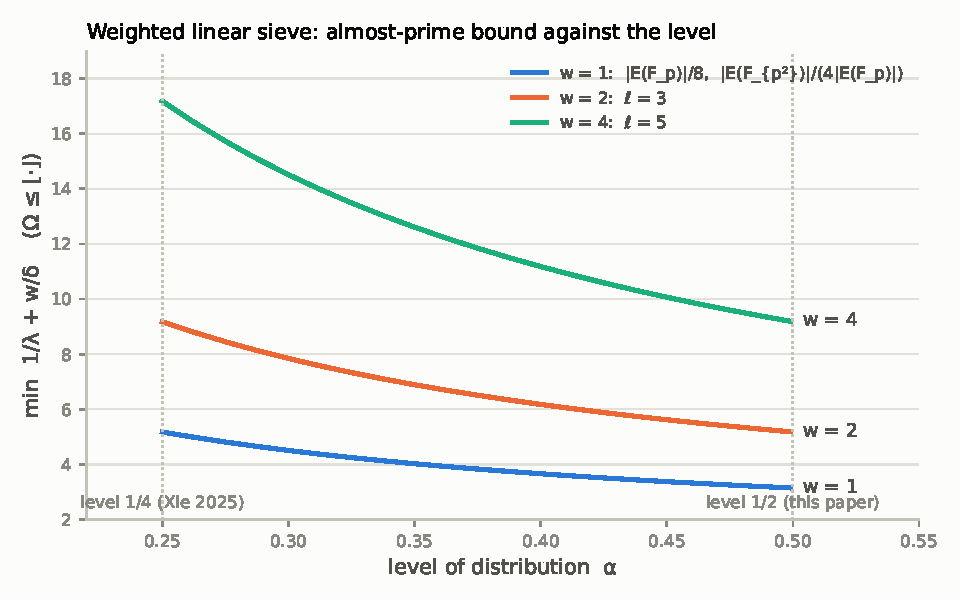
\includegraphics[width=0.82\textwidth]{level_vs_bound.pdf}
\caption{The almost-prime bound $\min_{\theta,\delta}(1/\lambda+w/\delta)$ of the weighted linear sieve \cite[(4.7)--(4.9)]{Xie} as a function of the level of distribution $\alpha$, with $\lambda$ chosen so that $G(\theta,\delta,\lambda)=0$ and $F$, $f$ continued beyond their closed-form ranges by the delay-differential equations $(sF(s))'=f(s-1)$, $(sf(s))'=F(s-1)$. The weight $w$ is $1$ for $|E(\F_p)|/8$ and $|E(\F_{p^2})|/(4|E(\F_p)|)$, and $\ell-1$ for $|E(\F_{p^\ell})|/|E(\F_p)|$. The bound on $\Omega$ is the integer part. Floating-point exploration (\texttt{scan\_levels.py} in the repository described at the end of the paper); the values used in Corollary~\ref{cor:Xie} are certified separately.}
\label{fig:level}
\end{figure}

\section{Remarks on the remaining parts of the proof in \cite{IJU}}\label{sec:rest}

Since \cite[Remark~4.1]{Xie} casts doubt on \eqref{eq:IJU}, we record the points of \cite{IJU} that we have checked besides the level of distribution.

\subsection{Proposition 5.1 of \cite{IJU}}
This is the Bombieri--Vinogradov theorem for $\Om(x)$, i.e.\ hypothesis (i) for $R_{\mathcal B}$. Its proof in \cite{IJU} is a standard dispersion argument: after separating the variable $\pi_3$ from $\pi_1\pi_2$ by a partition of $[z,y)$ into intervals $[z_k,z_k(1+\delta))$, $\delta=L^{-A-2}$, the character sums factor as $A_k(\chi)B_k(\chi)$ with $A_k(\chi)=\sum_{\N(\pi_3)\in[z_k,z_k(1+\delta))}\chi(\pi_3)$; after reduction to primitive characters, conductors of norm $>R=L^{O_A(1)}$ are treated by the large sieve for $\Z[i]$ \cite[Lemma~5.5]{IJU} (Huxley \cite{Hux68}) and Cauchy's inequality, and conductors of norm $\le R$ by \cite[Lemma~5.2]{IJU}. We have re-derived the proposition in full; two comments are in order.

(a) The hypothesis (5.3) of \cite[Lemma~5.2]{IJU} is attributed there to \cite[Proposition~3.2]{IJU}, which is an average over moduli and does not give a bound for an individual modulus. What is needed is a Siegel--Walfisz theorem for primary Gaussian primes: for every $C>0$, every odd ideal $\mathfrak f\ne(1)$ with $\N(\mathfrak f)\le(\log t)^{C}$ and every primitive character $\chi$ modulo $\mathfrak f$,
\begin{equation}\label{eq:SW}
\sum_{\substack{\pi\ \mathrm{primary}\\ \N(\pi)\le t}}\chi(\pi)\ll_C t\exp(-c\sqrt{\log t}).
\end{equation}
This holds (with an ineffective constant, as usual). Indeed, reduction modulo $2+2i$ maps the unit group $\{\pm1,\pm i\}$ isomorphically onto $(\Z[i]/(2+2i))^\times$, so there is exactly one character $\psi$ modulo $2+2i$ with $\psi(u)=\chi(u)^{-1}$ for all units $u$. The character $\chi\psi$ of $(\Z[i]/\mathfrak f(2+2i))^\times$ is trivial on the units, hence is a ray class character modulo $\mathfrak f(2+2i)$, i.e.\ a function on ideals; and for an odd prime ideal $\fp$ with primary generator $\pi$ we have $(\chi\psi)(\fp)=\chi(\pi)\psi(\pi)=\chi(\pi)$ because $\pi\equiv1\pmod{2+2i}$. Thus the left side of \eqref{eq:SW} is exactly $\sum_{\N(\fp)\le t}(\chi\psi)(\fp)$ (up to the prime $(1+i)$), and $\chi\psi$ is non-principal: its restriction to $(\Z[i]/\mathfrak f)^\times\times\{1\}$ is $\chi\ne\chi_0$. Now \eqref{eq:SW} is Lemma~16 of Mitsui \cite{Mit} (equivalently, the Theorem at the end of \cite[\S1]{Mit}): for a fixed number field $K$, a constant $C>0$, and a character $\chi$ of the ray class group modulo $\fq$ with $\N(\fq)\le(\log t)^{C}$,
\[
\sum_{\N(\fp)\le t}\chi(\fp)=E(\chi)\int_2^t\frac{\dd u}{\log u}+O\bigl(t\exp(-c\sqrt{\log t})\bigr),
\]
where $E(\chi)=1$ if $\chi$ is principal and $0$ otherwise, and $c>0$ and the implied constant depend only on $K$ and $C$; the Siegel-type zero-free region for real characters that this requires is \cite[Lemma~11]{Mit} (see also Fogels \cite{Fog} and Hinz \cite{Hinz}). In the proof of \cite[Proposition~5.1]{IJU} the hypothesis (5.3) is only used for moduli of norm $\le R\cdot\Delta^{-6}=L^{O_A(1)}$, so \eqref{eq:SW} suffices.

(b) For the prime variable $\pi_3$ the coprimality condition $(\pi_3,\fa)=1$ in \cite[(5.5)]{IJU} is trivial: $\N(\pi_3)\ge z$ exceeds the norm of any prime factor of a modulus of norm $\le L^{O(1)}$, so $(\pi_3,\fa)\neq1$ means $\pi_3\mid\fa$, which happens for at most $\omega(\fa)\ll L$ primes. Hence \cite[Lemma~5.2]{IJU} can be replaced by \eqref{eq:SW} directly, and the bound for the small conductors is $\ll xRL^{2}\cdot L^{-C'}$ for any $C'$. For the large conductors one obtains, exactly as in \cite[(5.8)]{IJU}, the bound $x^{1/2}L^{O(1)}\bigl(Q+y^{1/2}+(x/z)^{1/2}+x^{1/2}/R\bigr)$, which is $\ll xL^{-A}$ for $Q=x^{1/2}L^{-B}$ and suitable $B,R$. The exponents $1/8$ and $1/3$ enter only through $y^{1/2}x^{1/2}=x^{2/3}$ and $(x/z)^{1/2}x^{1/2}=x^{15/16}$.

\subsection{Minor points}
In the derivation of \cite[(5.9)]{IJU} the condition $(\omega,\fa)=1$ is removed from the main term; this costs $\Phi(\fa)^{-1}\#\{\omega:(\omega,\fa)\ne1\}$ per modulus, which is why the weight $\Phi(\fa)^{-1}$ must be kept in the sum over $\fa$ (as above); without it the sum would be of size $xQ/z$. The elements of $\mathcal B(x)$ are odd (not ``divisible by $2$'' as stated on \cite[p.~830]{IJU}), which is what is used: the sieve for $W_3$ runs over odd primes $p<\sqrt x$, and $\prod_{2<p<\sqrt x}(1-g(p))=(1-g(2))^{-1}\cdot\frac{\log z}{\log\sqrt x}\,V(z)(1+o(1))=\frac12V(z)(1+o(1))$ by \cite[(3.10)]{IJU} and $g(2)=\frac12$. The constants $\frac12e^{\gamma}\log 6$ in \cite[(4.3)]{IJU} (the sum over $p_0$ runs over split primes only, which have density $\frac12$ among all primes, with $g(p_0)\sim 2/p_0$) and $c<0.36308373$ in \cite[(5.10)]{IJU} were recomputed. The Chen-type weight \cite[(2.2)]{IJU} is the classical one: an element $a$ of $\mathcal A(x)$ coprime to $2P(z)Q(z)$ with positive weight is either $P_2$ or not square-free, because $a\le x/8$ has at most one prime factor $\le y$ unless two such factors give weight $\le 0$, and a square-free $a$ with exactly one prime factor $\le y$ and at least three prime factors is of the form $p_1p_2p_3$ counted by $W_3$ (four factors would exceed $x^{1/8}\cdot x=x^{9/8}$); the non-square-free elements are $\ll x\log x/(z\log z)$ in number.

\section*{Data and code availability}
The scripts behind the numerical statements of this note are available at
\begin{center}
\url{https://github.com/Ruqing1963/cm-orders-level-half}
\end{center}
(tag \texttt{v1.0}); the manuscript is archived at Zenodo, \href{https://doi.org/10.5281/zenodo.23428952}{doi:10.5281/zenodo.23428952} (record \url{https://zenodo.org/records/23428952}, version v1, 17 October 2026). The scripts comprise
the interval-arithmetic evaluation of $G$ in Section~\ref{sec:appl} (\texttt{certify\_G.py}, exact rational parameters, closed form), the computation of the constants of Section~3.4, the exploration of Figure~\ref{fig:level} (\texttt{scan\_levels.py}, with the resulting table), and a first-principles check of the bookkeeping of Section~\ref{sec:appl}. The latter script, \texttt{check\_omega\_distribution.py}, builds for $x=10^8$ the set $\Om(x)$ and the primary primes of norm $\le x$, verifies the identity \eqref{eq:ie} exactly for $p=5,13,17,29,37,41$, compares the divisor densities with $g(d)$, and measures the discrepancies $E(x;\alpha,\fa)$, which are of the size of the square root of the main term for all moduli tested.

\begin{thebibliography}{99}

\bibitem{Coj} A.~C. Cojocaru, \emph{Reductions of an elliptic curve with almost prime orders}, Acta Arith.\ \textbf{119} (2005), 265--289.

\bibitem{Fog} E.~Fogels, \emph{On the zeros of Hecke's $L$-functions I}, Acta Arith.\ \textbf{7} (1962), 87--106.

\bibitem{HR} H.~Halberstam and H.-E. Richert, \emph{Sieve Methods}, London Math.\ Soc.\ Monographs 4, Academic Press, London--New York, 1974.

\bibitem{Hinz} J.~G. Hinz, \emph{A generalization of Bombieri's prime number theorem to algebraic number fields}, Acta Arith.\ \textbf{51} (1988), 173--193.

\bibitem{Hux68} M.~N. Huxley, \emph{The large sieve inequality for algebraic number fields}, Mathematika \textbf{15} (1968), 178--187.

\bibitem{Hux71} M.~N. Huxley, \emph{The large sieve inequality for algebraic number fields III. Zero-density results}, J.\ London Math.\ Soc.\ (2) \textbf{3} (1971), 233--240.

\bibitem{IJU} H.~Iwaniec and J.~Jim\'enez Urroz, \emph{Orders of CM elliptic curves modulo $p$ with at most two primes}, Ann.\ Sc.\ Norm.\ Super.\ Pisa Cl.\ Sci.\ (5) \textbf{9} (2010), 815--832.

\bibitem{JU} J.~Jim\'enez Urroz, \emph{Almost prime orders of CM elliptic curves modulo $p$}, in: Algorithmic Number Theory (ANTS VIII), Lecture Notes in Comput.\ Sci.\ 5011, Springer, 2008, 74--87.

\bibitem{Joh} D.~Johnson, \emph{Mean values of Hecke $L$-functions}, J.\ reine angew.\ Math.\ \textbf{305} (1979), 195--205.

\bibitem{Kob} N.~Koblitz, \emph{Primality of the number of points on an elliptic curve over a finite field}, Pacific J.\ Math.\ \textbf{131} (1988), 157--165.

\bibitem{Mit} T.~Mitsui, \emph{Generalized prime number theorem}, Japan.\ J.\ Math.\ \textbf{26} (1956), 1--42.

\bibitem{Xie} L.~Xie, \emph{Almost prime orders of elliptic curves over prime power fields}, preprint, arXiv:2504.18732 (2025).

\end{thebibliography}

\end{document}
